\documentclass[border=10pt]{standalone}
\usepackage{tikz}
\usepackage{amsmath,amssymb}
\usepackage{xcolor}
\usetikzlibrary{arrows.meta,positioning,fit,calc}

\definecolor{usdcblue}{HTML}{2e6fb7}
\definecolor{usdtred}{HTML}{c75b4a}

\begin{document}

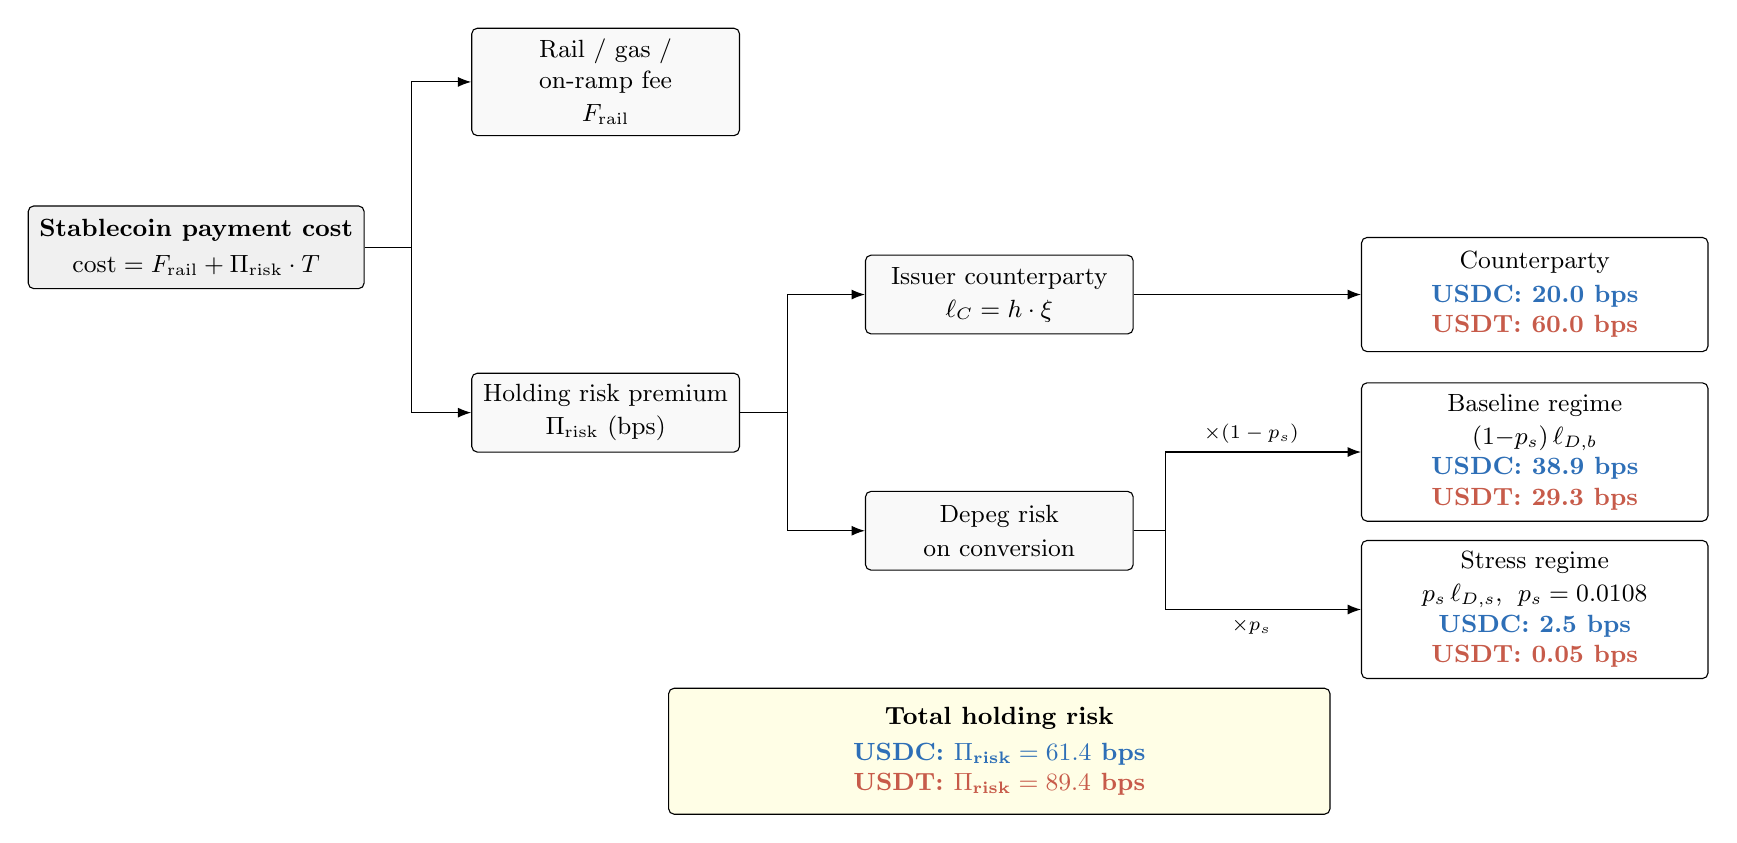
\begin{tikzpicture}[
  font=\small,
  every node/.style={align=center},
  rootbox/.style={rectangle, rounded corners=2pt, draw, fill=gray!12,
                  minimum width=3.8cm, minimum height=1.05cm, inner sep=4pt},
  branchbox/.style={rectangle, rounded corners=2pt, draw, fill=gray!5,
                    minimum width=3.4cm, minimum height=1.0cm, inner sep=4pt},
  leafbox/.style={rectangle, rounded corners=2pt, draw, fill=white,
                  minimum width=4.4cm, minimum height=1.45cm, inner sep=4pt},
  totalbox/.style={rectangle, rounded corners=2pt, draw=black, fill=yellow!10,
                   minimum width=8.4cm, minimum height=1.6cm, inner sep=6pt},
  >=Latex,
  edgelab/.style={font=\scriptsize, fill=white, inner sep=2pt}
]

% Root
\node[rootbox] (pay) at (0, 0)
  {\textbf{Stablecoin payment cost}\\[2pt]
   $\text{cost} = F_{\text{rail}} + \Pi_{\text{risk}} \cdot T$};

% First split
\node[branchbox] (fee)  at (5.2,  2.1) {Rail / gas /\\on-ramp fee\\[1pt]$F_{\text{rail}}$};
\node[branchbox] (hold) at (5.2, -2.1) {Holding risk premium\\[1pt]$\Pi_{\text{risk}}$ (bps)};

% Second split (from hold)
\node[branchbox] (cpty)  at (10.2, -0.6) {Issuer counterparty\\[1pt]$\ell_C = h \cdot \xi$};
\node[branchbox] (depeg) at (10.2, -3.6) {Depeg risk\\[1pt]on conversion};

% Third split (from depeg)
% Leaves on right
\node[leafbox] (cpty_leaf) at (17.0, -0.6)
  {Counterparty\\[1pt]
   \textcolor{usdcblue}{\textbf{USDC: 20.0 bps}}\\
   \textcolor{usdtred}{\textbf{USDT: 60.0 bps}}};

\node[leafbox] (base_leaf) at (17.0, -2.6)
  {Baseline regime\\[1pt]$(1{-}p_s)\,\ell_{D,b}$\\
   \textcolor{usdcblue}{\textbf{USDC: 38.9 bps}}\\
   \textcolor{usdtred}{\textbf{USDT: 29.3 bps}}};

\node[leafbox] (stress_leaf) at (17.0, -4.6)
  {Stress regime\\[1pt]$p_s\,\ell_{D,s}$, $\;p_s=0.0108$\\
   \textcolor{usdcblue}{\textbf{USDC: 2.5 bps}}\\
   \textcolor{usdtred}{\textbf{USDT: 0.05 bps}}};

% Edges - first split
\draw[->] (pay.east) -- ++(0.6,0) |- (fee.west);
\draw[->] (pay.east) -- ++(0.6,0) |- (hold.west);

% Edges - second split
\draw[->] (hold.east) -- ++(0.6,0) |- (cpty.west);
\draw[->] (hold.east) -- ++(0.6,0) |- (depeg.west);

% Edges - third split
\draw[->] (cpty.east)  -- (cpty_leaf.west);
\draw[->] (depeg.east) -- ++(0.4,0) |- node[edgelab, pos=0.72, above=1pt] {$\times (1-p_s)$} (base_leaf.west);
\draw[->] (depeg.east) -- ++(0.4,0) |- node[edgelab, pos=0.72, below=1pt] {$\times p_s$}     (stress_leaf.west);

% Total box at bottom
\node[totalbox] at (10.2, -6.4)
  {\textbf{Total holding risk}\\[2pt]
   \textcolor{usdcblue}{\textbf{USDC: $\Pi_{\text{risk}}=61.4$ bps}}\\
   \textcolor{usdtred}{\textbf{USDT: $\Pi_{\text{risk}}=89.4$ bps}}};

\end{tikzpicture}

\end{document}
